\documentclass[12pt]{amsart}
\usepackage[margin=1in]{geometry} 
\usepackage{amsmath,amsthm,amssymb,amsfonts}
\usepackage[pdftex]{graphicx}
\usepackage[utf8]{inputenc}
\usepackage{amsmath}
\usepackage{amssymb}
\usepackage{bm}
\usepackage{mathrsfs}

\newtheorem{theorem}{Theorem}[section]
\newtheorem{lemma}[theorem]{Lemma}
\newtheorem{proposition}[theorem]{Proposition}
\newtheorem{corollary}{Corollary}[theorem]

\theoremstyle{definition}
\newtheorem*{definition}{Definition}

\theoremstyle{remark}
\newtheorem*{note}{Note}



\newcommand{\N}{\mathbb{N}}
\newcommand{\R}{\mathbb{R}}
\newcommand{\Z}{\mathbb{Z}}

\newcommand{\Mod}[1]{\ (\mathrm{mod}\ #1)}

\setcounter{section}{-1}

\begin{document}
 
\renewcommand{\qedsymbol}{$\blacksquare$}
%Good resources for looking up how to do stuff:
%Binary operators: http://www.access2science.com/latex/Binary.html
%General help: http://en.wikibooks.org/wiki/LaTeX/Mathematics
%Or just google stuff
 
\title{A direct analysis of the NRTU cryptosystem}
\author{Quinn Murphey}
\begin{abstract}

NTRU, a public key lattice-based cryptosystem introduced in 1997, still lacks industry applications compared to RSA and elliptic curve cryptography. Now that NTRU is in the public domain we compare it to the current industry standards and show it's an advantage over them. Additionally, to cement its utility we show some of the most successful cryptanalysis techniques and preventative measures that can be taken to avoid known weaknesses.

%We describe NTRU, a public lattice-based cryptosystem. Then we demonstrate several published cryptanalysis techniques for NTRU and preventative measures. And finally, we compare NTRU directly to discrete logarithm cryptosystems such as RSA and Elliptic Curve ElGamal. 

%Put paper abstract here.  
%(Usually 3--5 sentences.  
%Should be self-contained, intelligible to a peer reader not familiar with the specific topic of the paper, and as descriptive as possible.)
\end{abstract}
\maketitle

\section{Introduction}

In this paper we will be covering the basics of the NTRU cryptosystem \cite{NTRUpatent}, identifying its weaknesses, and comparing it to other cryptosystems such as RSA, McElise, and Elliptic Curve ElGamal. Despite being almost 20 years since NTRU was introduced, and the advantages it provides computationally, other systems such as RSA and Elliptic Curve parallels are the current industry standard. Now that NTRU is public domain (2017), we urge security departments to incorporate NTRU in place of other asymmetric cryptosystems for the reasons which follow.

\section{Preliminaries}

In order to explain the cryptosystem and NTRU cryptanalysis we need to cover some definitions relevant theorems regarding lattices. \cite{DecadeSum}
\begin{definition}\label{def:Lattice}
Let $\bm{v}_1,\dots,\bm{v}_n\in\R^n$ be a set of linearly independent vectors. The \textit{Lattice $\mathcal{L}$ generated by} $\bm{v}_1,\dots,\bm{v}_n$ is the set of linear combinations of $\bm{v}_1,\dots,\bm{v}_n$ with coefficients from $\Z$, $$\mathcal{L} = \{ a_1\bm{v}_1 + a_2\bm{v}_2 + \dots + a_n\bm{v}_n : a_1,a_2,\dots,a_n\in\Z\}.$$
\end{definition}

We require for the generating set of $n$ vectors, which we call the \textit{basis}, to be linearly independent so that the lattice is the same dimension as the Euclidean space where it resides, or in other words, we require the lattice to be \textit{Full Rank}.\\

Let $V$ be the column matrix whose rows are vectors $\bm{v}_1,\dots,\bm{v}_n$,
\begin{equation*}
    V = 
    \begin{bmatrix}
        \bm{v}_1\\
        \bm{v}_2\\
        \vdots\\
        \bm{v}_{n-1}\\
        \bm{v}_n
    \end{bmatrix}
\end{equation*}

\begin{proposition}
Any two bases for a lattice $\mathcal{L}$ are related by a matrix $U$ with integer coefficients and determinant equal to $\pm 1$. \cite{DecadeSum}

This relation is defined as $W = UV$ where $\bm{w}_1,\dots,\bm{w}_n$ are the rows of $W$.
\end{proposition}
\begin{proof}
    Suppose that $\bm{v}_1,\dots,\bm{v}_n$ is a basis for a lattice $\mathcal{L}$ and that $\bm{w}_1,\dots,\bm{w}_n\in\mathcal{L}$. Then we can write each $\bm{w}_i$ as an integral linear combination of our basis like
    \begin{align*}
        \bm{w}_1 &= a_{11}\bm{v}_1 + a_{12}\bm{v}_2 + \dots + a_{1n}\bm{v}_n\\
        \bm{w}_2 &= a_{21}\bm{v}_1 + a_{22}\bm{v}_2 + \dots + a_{2n}\bm{v}_n\\
        \vdots \text{ }&\qquad\qquad\qquad \vdots\\
        \bm{w}_n &= a_{n1}\bm{v}_1 + a_{n2}\bm{v}_2 + \dots + a_{nn}\bm{v}_n
    \end{align*}
    In other words, $A = (a_{i,j})_{i=j=1}^n$ is the matrix such that $W = AV$, where $W,V$ are the respective column matrices of vectors $\bm{v}_i$ and $\bm{w}_i$ respectively.
    
    In order for $\bm{w}_1,\dots,\bm{w}_n$ to be a basis for $\mathcal{L}$ we must be able to represent each $v_i$ as a integral linear combination of $\bm{w}_1,\dots,\bm{w}_n$. This gives us $V = A^{-1}U$, where $A^{-1}$ must have all integer entries. Since the determinant of a integer matrix is an integer and 
    $$1 = \det(I) = \det(AA^{-1}) = \det(A)\det(A^{-1}),$$
    and 1 and -1 are the only units in the integers, we have the condition that $\det(A)=\pm 1$ or $A \in GL_{n}(\Z).$
\end{proof}

\begin{note}
We can easily obtain a ``random'' matrix $U$ by multiplying many elementary matrices $U_1\dots,U_k$ with determinant $\pm1$ together. $U = U_1U_2\dots U_k$
\end{note}

\begin{definition}
Let $\mathcal{L}$ be a $n$ dimensional lattice, and let $\bm{v}_1,\dots,\bm{v}_n$ be a basis for $\mathcal{L}$. The \textit{fundamental domain} $\mathcal{F}$ of $\mathcal{L}$ corresponding to this basis is defined 
$$\mathcal{F}(\bm{v}_1,\dots,\bm{v}_n) = \{ t_1\bm{v}_1, t_2\bm{v}_2 + \dots + t_n\bm{v}_n : 0\leq t_i < 1\}$$

\noindent Additionally, every vector $\bm{w}\in\mathbb{R}^n$ can be written \cite{DecadeSum}
$$\bm{w} = \bm{t} + \bm{v} \quad \text{for a unique } \bm{t}\in\mathcal{F} \text{ and a unique } \bm{v}\in\mathcal{L}$$
\end{definition}

\noindent We use the notation Vol($\mathcal{F}$) to denote the volume of the parallelepiped formed by the $n$ basis vectors.\\

To measure the orthogonality of a basis we use the following:
\begin{definition}
(Hadamard's Ratio) \cite{DecadeSum}. Let $\mathcal{L}$ be a lattice, and let $\bm{v}_1,\bm{v}_n$ be a basis for $\mathcal{L}$. $0< \mathcal{H}(\bm{v}_1,\dots,\bm{v}_n) \leq 1$ such that 
$$\mathcal{H}(\bm{v}_1,\dots,\bm{v}_n) = \frac{\text{Vol}(\mathcal{F})}{\lvert\lvert\bm{v}_1\rvert\rvert\text{ } \lvert\lvert\bm{v}_2\rvert\rvert \dots \lvert\lvert\bm{v}_n\rvert\rvert}$$
\end{definition}

\noindent The closer this ratio is to 1, the more orthogonal the basis is.\\

Next, we will introduce the two fundamental computational problems of lattice-based cryptography:

\textbf{The Shortest Vector Problem} (SVP): Find a shortest nonzero vector in a lattice $\mathcal{L}$. (Minimize $\lvert\lvert \bm{v}\rvert\rvert.$)

\textbf{The Closest Vector Problem} (CVP): Given a vector $\bm{w}\in\R^n$ that is not in a lattice $\mathcal{L}$, find a vector $\bm{v}\in\mathcal{L}$ that is closest to $\bm{w}$. (Minimize $\lvert\lvert \bm{w}-\bm{v}\rvert\rvert$.)

\begin{note}
There may be more than one shortest nonzero vector hence why the SVP asks for ``a'' shortest vector.
\end{note}

Both of these problems become computationally difficult as the dimension $n$ grows. Another benefit of the SVP versus the traditional Discrete Logarithm Problem (DLP) is resistance against the quantum Shor's Algorithm. 

Now we can look at the specifics of NTRU itself.

\section{The NTRU Algorithm}

The NTRU cryptosystem presents itself as a cryptosystem over polynomial convolution rings ($\Z[x]/\langle x^N - 1\rangle$). However, as we will discuss later, it can be rephrased in terms of the SVP problem we mentioned earlier. 
\textit{Note:} Much of this process is adapted directly from the original paper by Hoffstein, Pipher, and Silverman \cite{NTRUpatent}.

\subsection{Notation and parameters} 
NTRU has four public parameters ($N,K,p,q$) and four sets of polynomials $\mathscr{L}_g,\mathscr{L}_f, \mathscr{L}_\phi,\mathscr{L}_m \subset R = \Z[x]/\langle x^N - 1\rangle$. \cite{NTRUpatent} We will write each $F\in R$ as a vector 
$$F = \sum_{i=0}^{n-1}F_ix^i = [F_0,F_1,\dots,F_{n-1}].$$
Due to the properties of multiplication in a convolution ring, we denote multiplication of two polynomials $F$ and $G$ in $R$ as $F\circledast G = H$. This operation can be defined explicitly as
\begin{align}
    F\circledast G = H \qquad \text{with}\quad H_k = \sum_{i+j\equiv k \Mod{N}}F_iG_j
\end{align}
This is because in our ring, $x^N = 1$ instead of $0$ in normal polynomial rings. When we multiply two polynomials mod $q$ we reduce the coefficients mod $q$
\subsection{Key Creation}
To create a NTRU key, we randomly chooses $K+1$ polynomials $f\in\mathscr{L}_f$ and $g_1,g_2,\dots,g_K\in\mathscr{L}_g$. The polynomial $f$ must have inverses modulo $p$ and $q$ denoted $F_p$ and $F_q$ respectively. Next, we compute 
\begin{equation}
    h_i \equiv F_q \circledast g_i\Mod{q} \qquad 1\leq i \leq K
\end{equation}
and let the list of polynomials $[h_1,h_2,\dots,h_K]$ be our public key.\cite{NTRUpatent}
\subsection{Encryption}
To encode a message $m\in\mathscr{L}_m$, we choose $K$ random polynomials $\phi_1,\dots,\phi_K\in\mathscr{L}_\phi$ and use the public key $[h_1,h_2,\dots,h_K]$ to compute 
$$e \equiv \sum_{i=1}^K p(\phi_i\circledast h_i) + m \Mod{p}.$$
$e$ is our cyphertext. \cite{NTRUpatent}
\subsection{Decryption}
In order to decrypt $e$ we first compute $a \equiv f \circledast e \Mod{q}$. Where the coefficients for $a$ are between $-q/2$ and $q/2$. Then we retrieve $m$ by computing \cite{NTRUpatent} 
\begin{equation}
    F_p\circledast a \Mod{p}
\end{equation}
\subsection{Decryption Proof}
Given appropriate parameter choice, there is an extremely high probability the decryption will give the original message. However due to the chance of failure we recommend using a few check bits. Additionally, if it's incorrect, it's likely we have $F_p\circledast a \Mod{p}$ equalling a shift of $m$ meaning 
$$F_p\circledast a \Mod{p} = m + x \Mod{q}$$
for some small integer $x$.\cite{NTRUpatent}

The polynomial $a$ satisfies
\begin{align*}
    a &\equiv f\circledast e = \sum_{i=1}^K f\circledast p(\phi_i\circledast h_i) + f\circledast m \Mod{q}\\
    &\equiv \sum_{i=1}^K (f\circledast p\phi_i\circledast F_q \circledast g_i) + f\circledast m \Mod{q} \qquad
    \text{by (2)}\\
    &\equiv \sum_{i=1}^K (p\phi_i\circledast g_i) + f\circledast m \Mod{q}.
\end{align*}
Considering this last polynomial, $\sum_{i=1}^K (p\phi_i\circledast g_i) + f\circledast m$, we can choose parameters such that all the coefficients lie between $-q/2$ and $q/2$ such that reducing modulo $q$ doesn't change the polynomial at all. Therefore we can look at $a$ as exactly
\begin{align*}
    a = \sum_{i=1}^K (p\phi_i\circledast g_i) + f\circledast m
\end{align*}
Reducing $a$ modulo $p$ gives us exactly $f\circledast m \Mod{p}$, and multiplying by $F_p$ gives us our message $m$ \cite{NTRUpatent}. In section 5 we will discuss parameter choice such that this is true at an arbitrary probability.

\section{A collection of attacks on the NTRU system}

In this section, we will cover three cryptanalysis techniques for attacking the NTRU cryptosystem other than the traditional LLL reeducation algorithm, and in the next section, we will discuss protection from these attacks by parameter choice.

\subsection{Reduced memory meet-in-the-middle attack} 

The attack described in \cite{ManInMiddle} is an attack based around the classic Man-in-the-middle attack used throughout all cryptography. To aid the attacker we will let $K = 1$.

An NTRU encoded message looks like $e \equiv \phi\circledast h + m\Mod{q}$. Briefly, one can split $f$ if half such that $f = f_1 + f_2$ and one can find those $f_1,f_2$ by looking for $f_1\circledast e$ approximately the same as $-f_2\circledast e$. Hence to obtain a security value of $2^{80}$ we must choose our polynomials from sets of about $2^{160}$.

\subsection{A chosen-ciphertext attack} 
The attack described in \cite{ChosenCipherAttack} is based around choosing a ciphertext to decrypt using a decryption oracle such that the decryption may allow us to calculate the secret key. We will start with the low-security attack, then build up to the high-security parameter attack. This attack is solely focused on the case where $K=1$ and $g,f$ are both ternary polynomials where $f$ has one more 1 than -1 and $g$ has the same number of both.

We will first show the effects of decrypting a ciphertext of the form $ch+c$, where $c$ is an integer divisible by $p$ such that $c<q/2$ and $2c>q/2$. The decryption algorithm first obtains $$a\equiv f\circledast ch + cf \equiv cg+ cf \Mod{q}.$$
where $g$ and $f$ both have coefficients equal to -1,0, or 1. Hence $a$ has coefficients equal to $0,c,-c,2c,$ or $-2c$. When reducing, only the $2c$ and $-2c$ terms must be reduced. if we assume that only one coefficient in $a$ is $\pm 2c$, say $a_i = 2c$, then the value of $a$ mod $q$ is $cg+cf -qx^i\circledast F_p \Mod{p}$. The deciphering process then outputs
$$cg\circledast F_p + c - qx^i\circledast F_p \equiv -qx^i\circledast F_p\Mod{p}$$
since $c$ is a multiple of $p$. Since gcd($p,q$) = 1, we can compute the inverse of this and find $f/x^i \Mod{p}$, since all the values are $-1,0$ or 1, this is the true value of $f/x^i$. Looking at the NTRU system, we also see that $(f/x^i, g/x^i)$ and $(f,g)$ are equivalent keys so we have broken the NTRU system. However this only works when $f$ and $g$ only have one intersection defined 
$$ k = \sum k_ix^i$$
where
$$k_i = \begin{cases} 
      1 \text{ if } f_i=g_i=1\\
      -1 \text{ if } f_i=g_i=-1\\
      0 \text{ otherwise.}
   \end{cases}$$
\\

The expected number of collisions between a random $f$ and $g$ can be approximated by 
$$\frac{(2d_f-1)d_g}{N}.$$
Where $d_f$ denotes the number of 1's in $f$ and likewise for $g$ and $N$ is the dimension of the convolution ring. 

We can see heuristically that this works well for low parameters but doesn't work on harder lattices.

However, we can reduce the average number of collisions (appearances of coefficients greater than $q/2$ in $a$ since we want exactly one) by using the ciphertext 
$$chx^{i_1}+\dots + chx^{i_n} + cx^{j_1} + \dots + cx^{j_m},$$
where $c$ is a multiple of $p$ such that 
$$(n+m-1) < q/2 \qquad (n+m)c > q/2.$$

We use the heuristic approximate provided in \cite{ChosenCipherAttack} of the number of collisions as
$$\frac{2d_f^md_g^n}{N^{n+m-1}}$$
to choose an $n$ and $m$ such that this is minimized while $m,n < N$.

This attack abuses the decryption oracle to gain information about $f$ through very specific ciphertext choice.  While the best defense is to not share decryptions of any ciphertext, another way to avoid the implications of this attack are choosing $f$ and $g$ such that they have at least several collisions always instead of completely random.

\subsection{Learning a parallelepiped} 
This attack described in \cite{LearningAttack} is based around using a gradient descent algorithm paired with a collection of vectors uniformly distributed throughout the fundamental domain to approximate the chosen basis of the lattice. The attack is aimed at the NTRU-Sign algorithm rather than the NTRU-Encrypt algorithm but we are discussing it as a precaution for a potential future NTRU-Encrypt analysis.

The weakness found in NTRU-Sign was the approximately uniform distribution of signatures across the fundamental domain and the existence of $N$ possible keys which perform the same thing ($x^if \equiv f$). This turns the SVP into the Hidden Parallelepiped Problem, which is the problem of finding the direction of $n$ vectors. This problem is known to be solvable in polynomial time. We will show one such approximate solution presented in \cite{LearningAttack} below.\\

First, we will attempt to morph the uniform distribution over the parallelepiped into a uniform distribution over a hypercube.

\begin{lemma}[\textbf{Hypercube Transformation}]\label{lem:hypercubeTransformation}
Let $V\in GL_n(\R)$ be the basis matrix of our lattice. Let $G = V^tV \in GL_n(\R)$. And let $L$ be the Cholesky factor of $G^{-1}$, or the unique lower-triangular matrix such that $G^{-1}=LL^t$. Then the matrix $C=VL\in GL_n(\R)$ satisfies the following: 
\begin{enumerate}
    \item $C$ is an orthogonal matrix and $\mathcal{F}(C)$ (the fundamental domain of the rows of $C$) is a unit hypercube.
    \item If $\bm{v}$ is uniformly distributed over $\mathcal{F}(V)$, then $\bm{c} = \bm{v}L$ is uniformly distributed over the hypercube $\mathcal{F}(C)$.
\end{enumerate}
\end{lemma}
\begin{proof}
    For the first claim, we have 
    \begin{align*}
        CC^t = VLL^tV^t=VV^{-1}V^{-t}V^t = I
    \end{align*}
    so $C$ is orthonormal
    
    For the second claim we let $\bm{v}$ be uniformly distributed over $\mathcal{F}(V)$. Then we can write $\bm{v}=\bm{x}V$ where $\bm{x}$ is uniformly distributed over $[-1,1]^n$. It follows that $\bm{v}L =\bm{x}VL=\bm{x}C$ which is uniformly distributed over $\mathcal{F}(C)$.
\end{proof}

We can approximate the matrix used in Lemma \ref{lem:hypercubeTransformation} $G = V^tV$ as follows
\begin{lemma}[\textbf{Covariance Matrix Leakage}]\label{lem:covarianceLeak}
Let $V\in GL_n(\R)$ be the masis matrix of our lattice. Let $\bm{v}$ be chosen from the uniform distribution over $\mathcal{F}(V)$. Then the covariance matrix of the distribution $U(\mathcal{F(V)}$ is $V^tV/3$
\end{lemma}
\begin{proof}
Follows from $\bm{v}=\bm{x}V$ where $\bm{x}\in U([-1,1]^n)$ so $\bm{v}^t\bm{v} = V^t\bm{x}^t\bm{x}V$. The expected value of $\bm{x}^t\bm{x}$ is $I_n/3$ so the expected value of $\bm{v}^t\bm{v}$ is $V^tV/3$
\end{proof}

We can take the average of $\bm{v}^t\bm{v}$ over our samples from $U(\mathcal{F}(V))$ and multiply by 3 to get an approximation of $V^tV$.

Since $\widetilde{C} \approx VL$, it will be very close to some orthogonal matrix $C$ and $\mathcal{F}(\widetilde{C})$ distribution will be close to the uniform distribution of some unit hypercube. We will use one last lemma to construct a gradient descent algorithm to approximate $V$. \textit{Note:} C is orthonormal which means each of its column vectors lies on the unit hypersphere.

\begin{lemma}\label{lem:localMin}
Let $C = [\bm{c}_1,\dots,\bm{c}_n]\in O_n(\R)$. Then the global minimum of the 4th moment of $\mathcal{F}(C)$ over a vector $\bm{w}$ on the unit sphere of $\R^n$ is obtained uniquely at $\pm \bm{c}_1, \pm \bm{c}_2,\dots,\pm \bm{c}_n$. There are no other local minima.
\end{lemma}
\begin{proof}
    See \cite{LearningAttack}, uses lagrange multipliers to find that the minima $\bm{w}$ must satisfy $\langle \bm{c}_i, \bm{w} \rangle$ equals either 0 or $\sqrt{\alpha}$ for some $\alpha$. And we can find that the only $\bm{w}$ which satisfies this is the vector which is orthogonal to all but one $\bm{c}_i$ so $\bm{w}=\pm\bm{c}_i$.
\end{proof}

We can repeatedly run a gradient descent algorithm with randomized starting locations to find every $\pm\bm{c}_1,\dots,\pm\bm{c}_n$ and construct our true orthonormal $\pm C$. Next, using our approximation $\widetilde{G}$ we calculate $\widetilde{L}^{-1}$, the inverse of the Cholesky factor of $\widetilde{G}$. Since $V = CL^{-1}$, we have $\pm V \approx \pm C\widetilde{L}^{-1}$ which experimentally provides a good enough approximation to round each of the entries to the nearest integer to get $V$ at a high probability. To increase the probability, all we need is more sample signatures to better approximate $G$.

\section{Choosing Parameters}

    As we have seen in section 3, each of these attacks narrows down our set of ``safe'' parameters to choose from. In this section we will summarize the findings in \cite{NTRUpatent,ChosenCipherAttack,ManInMiddle,Parameters,NguyenThesis} on safe and efficient parameter choice.
    
    NTRU has 4 public parameters ($N,K,p,q$) and 4 sets of polynomials ($\mathscr{L}_f,\mathscr{L}_g,\mathscr{L}_\phi,\mathscr{L}_m$) in $\Z[x]/\langle x^n - 1\rangle $ which we will explain below with the single integer $d$. $N$ represents the dimension of the underlying convolution polynomial ring. $K$ represents the length of our public key and length of the sum during encryption. For all purposes we can let $K = 1$. $p$ and $q$ are integers which we will define later. Ring elements from $\Z/q\Z$ are read as their representatives from $[-q/2,q/2]$. 
    
    \begin{definition}[Ternary Polynomials]
    A ternary polynomial allows for incredibly fast computation, because multiplication of polynomials becomes repeated addition and subtraction of $1$, so we will be using them frequently for our polynomial spaces. We set the notation \cite{Parameters}:
    \begin{align*}
        \mathcal{T}_N &= \{ \text{Ternary polynomial of degree } N\}\\
        \mathcal{T}_N(d,e) &= \{ \text{Ternary polynomial of degree } N \text{ with exactly $d$ ones and $e$ minus ones}\}
        \end{align*}
    \end{definition}
    
    For convince and security, $d$ is a integer located around $N/3$ but no greater than $N/2$ so that $\mathcal{T}_n(d,d)$ is nonempty. We then let $\mathscr{L}_g=\mathscr{L}_\phi =\mathcal{T}_N(d,d)$ and $\mathscr{L}_f\subset\mathcal{T}_N(d-1,d)$ such that each $f\in\mathscr{L}_f$ is invertible modulo $p$ and $q$ shown below. 

    First we choose $N$ and $p$ to both be arbitrary primes based on the desired strength of the system. Then we choose random $d$ around $N/3$ but no greater than $N/2$. Then, let $q$ be coprime to $p$ such that $q>(6d+1)p$. Therefore, the decryption step will always succeed. (example parameters shown below)
    \begin{proof}
        Consider the polynomial 
        $$a \equiv p\phi\circledast g + f\circledast m \Mod{q}$$
        computed exactly in $\Z[x]$ rather than modulo $q$. We can see that the largest magnitude of any coefficient is $p\cdot 2d +(2d+1)\frac{1}{2}p=(3d+\frac{1}{2})p$. And since we let $p>(6d+1)p$, we can raise this up to it's representation in $[-q/2,q/2]$ exactly. Therefore the message is preserved.
    \end{proof}
    
    Therefore given the parameters constraints shown by Figure 1, we are certain that this encryption scheme will always work.

    \begin{figure}
        \begin{tabular}{c|c}
    \hline  $N$   &   \text{Prime and arbitrarily large, secure around 401}  \\
            $K$  &   \text{For simplicity, let $K=1$}    \\
            $p$   &   \text{Arbitrary small prime}    \\
            $d$   &   \text{Random number nearby $N/2$}    \\
            $q$   &   \text{gcd($q,p$)=1 and $q>(6d+1)p$}    
        \end{tabular}
        \caption{Parameter Choice}
        \label{fig:1}
    \end{figure}
    
    For security against the chosen ciphertext attack, you can verify that your $f\in\mathcal{T}(d+1,d)$ and $g\in\mathcal{T}(d,d)$ have many collisions, but it is more practical to just conceal decrypted messages.
    
    Some example industry strength parameters suggested in \cite{Parameters} for $2^{192}$ estimated security level are shown in Figure 2

\section{Conclusion}

\begin{figure}
    \begin{tabular}{|c|c|}
\hline  $N$     &   593  \\\hline
        $K$     &   1    \\\hline
        $p$     &   3    \\\hline
        $d$     &   197  \\\hline
        $q$     &   2048 \\\hline
    \end{tabular}
    \caption{Parameter choices for $2^{192}$ security estimate \cite{Parameters}}
    \label{fig:exampleParam}
\end{figure}

\begin{figure}
    \begin{tabular}{|c|c|c|c|}
        \hline              &   NTRU        &   RSA     &   McElise \\\hline
        Key Size            &   $N$         &   $N$     &   $N^2$   \\
        Encryption Speed    &   $N\log N$   &   $N^2$   &   $N^2$   \\
        Decryption Speed    &   $N\log N$   &   $N^3$   &   $N^2$   \\
        Message Expansion   &   2-1         &   1-1     &   2-1     \\\hline
    \end{tabular}
    
    \caption{NTRU vs RSA and McElise \cite{NTRUpatent}}
    \label{fig:DirectComparison}
\end{figure}

\begin{figure}
    \centering
    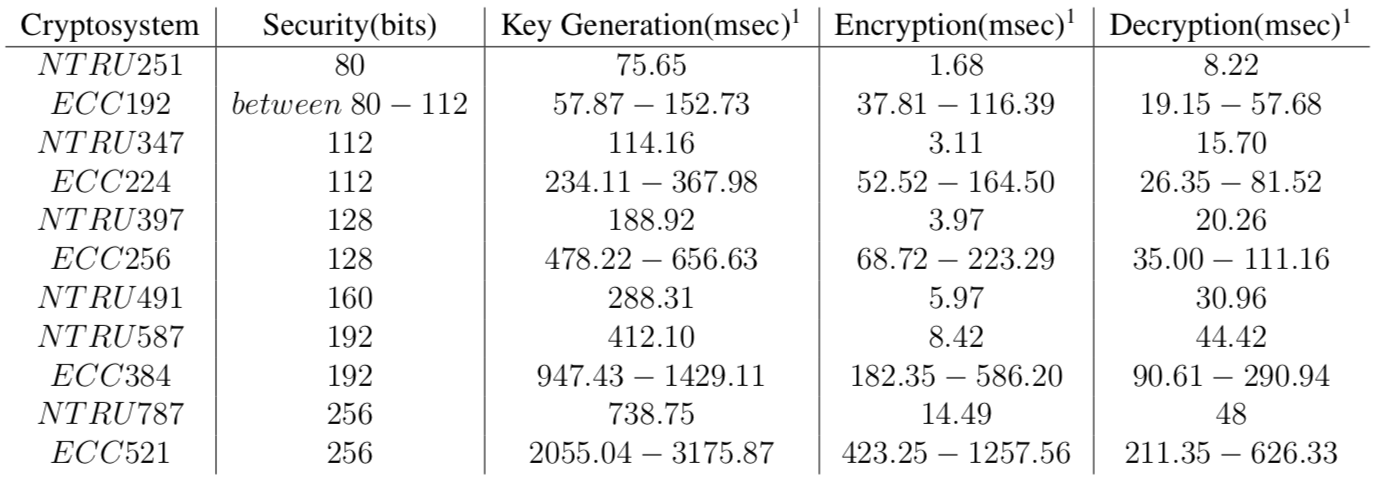
\includegraphics[width=\textwidth]{NTRUvsECC.png}
    \caption{NTRU experimentally compared with EC ElGamal\cite{NguyenThesis}}
    \label{fig:4}
\end{figure}

In this paper we covered the basics of the lattice-based cryptosystem introduced in 1997 known as NTRU. Then, looking throughout the literature for attacks and parameter choice we can make a much more educated comparison of security versus other modern cryptosystems. Additionally we looked at a lattice attack on NTRU-Sign in order to point out some weaknesses found in the symmetry of the convolution polynomial rings.

Looking at the analysis done in \cite{NTRUpatent} (Figure 3), where $N$ represents a function of security and message length, we can see that NTRU beats both RSA and McElise cryptosystems in mathematical complexity and in practical application. Another additional benefit to NTRU over the others is the fact that each operation in NTRU is an addition of polynomials (because of our usage of ternary polynomials) which speeds up the process drastically. Not only does it have fewer operations but also faster individual operations. 

Another paper \cite{NguyenThesis} covers an experimental analysis of NTRU and Elliptic Curve ElGamal shown in Figure 4 and found ``we discovered that the NTRU is much faster than the ECC with all levels of security.''  and found that ``NTRU is superior in comparison to the performance of minimum and maximum values of ECC timings''. By both of these separate analyses, we conclude that under proper parameter choice, the NTRU cryptosystem provides a much faster and more efficient alternative to RSA, McElise, and EC-ElGamal for the same security.

The other focus of this paper was to highlight that there is a large variety of possible attacks and due to this, we advocate for stricter parameter choice despite the consequential narrowing of the key set. This is because while it may speed up some brute force and collision attacks marginally, it removes large weaknesses that provide easy decryption methods for an attacker. 

Despite over 20 years of cryptanalysis research on NTRU, we have shown that the NTRU system remains unbroken and reins dominant in efficiency and speed over RSA and ECC. For these reasons, we urge the security industry to adopt NTRU in place of other, less effective algorithms according to the standardized parameter selection. This will allow for significantly less expensive security measures than currently in use.


\begin{thebibliography}{1}

\bibitem{NTRUpatent} Hoffstein, Jeffery, et al. PUBLIC KEY CRYPTO-SYSTEM METHOD AND APPARATUS. 27 June 2000. US-6,081,597

\bibitem{Parameters} Hoffstein, Jeff, et al. “Choosing Parameters for NTRUEncrypt.” Topics in Cryptology – CT-RSA 2017 Lecture Notes in Computer Science, 2017, pp. 3–18., doi:10.1007/978-3-319-52153-4\_1.

\bibitem{NguyenThesis} Nguyen, Hien Ba. “An Overview of the NTRU Cryptographic System.” San Diego State University, 2014. M.A. Thesis

\bibitem{ManInMiddle} Vredendaal, Christine Van. “Reduced Memory Meet-in-the-Middle Attack  against the NTRU Private Key.” LMS Journal of Computation and Mathematics, vol. 19, no. A, 2016, pp. 43–57.

\bibitem{ChosenCipherAttack} Jaulmes, Éliane, and Antoine Joux. “A Chosen-Ciphertext Attack against NTRU.” Advances in Cryptology — CRYPTO 2000 Lecture Notes in Computer Science, 2000, pp. 20–35., doi:10.1007/3-540-44598-6\_2.

\bibitem{LearningAttack} Nguyen, Phong Q., and Oded Regev. “Learning a Parallelepiped: Cryptanalysis of GGH and NTRU Signatures.” Journal of Cryptology, vol. 22, no. 2, 2008, pp. 139–160., doi:10.1007/s00145-008-9031-0.

\bibitem{DecadeSum} Peikert, Chris. \textit{A Decade of Lattice Cryptography}. Now Publishers, 2016.

\end{thebibliography}

\end{document}